\newchapstyle
\chapter{Theory}
\label{chap:theory}


%%% The '0pt' option ensures that no extra vertical space follows this epigraph,
%%% since there is another epigraph after it.
%\epigraph[0pt]{
%    Nature and nature's laws lay hid in the night; \\
%    God said `Let Newton be!' and all was light.
%}{Alexander Pope}
%
%\epigraph{
%    It did not last: the devil shouting `Ho. \\
%    Let Einstein be!' restore the status quo.
%}{Sir John Collings Squire}
%
%\begin{abstract}
%Lorem ipsum dolor sit amet, consectetur adipisicing elit, sed do eiusmod tempor incididunt ut labore et dolore magna aliqua. Ut enim ad minim veniam, quis nostrud exercitation ullamco laboris nisi ut aliquip ex ea commodo consequat. Duis aute irure dolor in reprehenderit in voluptate velit esse cillum dolore eu fugiat nulla pariatur. Excepteur sint occaecat cupidatat non proident, sunt in culpa qui officia deserunt mollit anim id est laborum.
%\end{abstract}

%% Start the actual chapter on a new page.
\newpage

\section{SQUIDs}

\begin{figure}
	\centering
	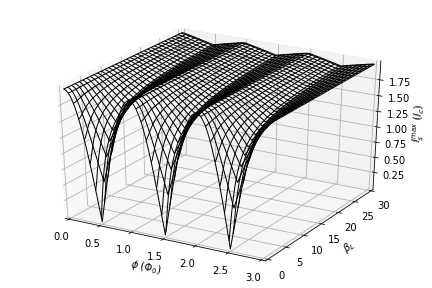
\includegraphics[width=0.5\linewidth]{./chapter-theory/figs-JJ/SQUID_betaL}
	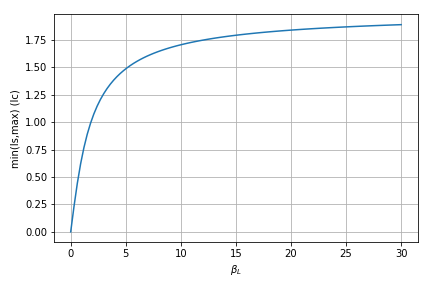
\includegraphics[width=0.4\linewidth]{./chapter-theory/figs-JJ/SQUID_betaL_I}
	\caption{Critical current modulation of SQUID for various screening factors $\beta_L$.}
	\label{fig:betaL}
\end{figure}

\section{Induced superconductivity and Josephson junctions}

\dropcap{T}{he} process of Andreev reflection at the interface between superconductors and normal metals lays the fundament for understanding how a Josephson junction works.
The process is sketched in Fig. \ref{fig:kdtmk}:
An electron impinging onto the super-normal interface from inside the normal region can only enter the superconductor in the form of a Cooper pair by being reflected as a hole with opposite spin and momentum.
Vice versa, a Cooper pair travelling towards the normal region will decay into an electron travelling forward, and annihilate a hole travelling backwards with spin opposite to that of the electron.
Inside the normal region, this will result in the formation of the so-called Andreev bound states (ABS).

\begin{figure}
	\centering
	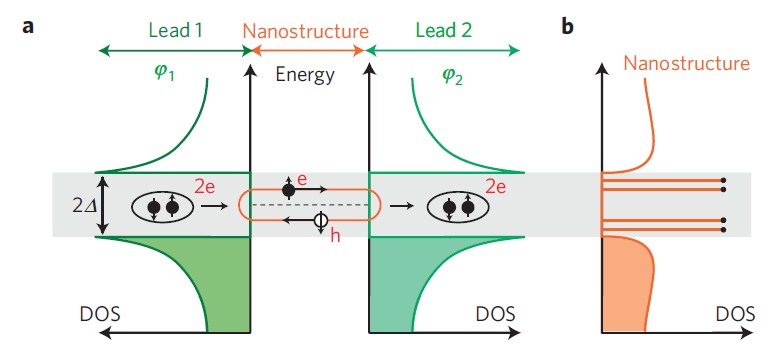
\includegraphics[width=0.7\linewidth]{./chapter-theory/figs-JJ/KDTMK}
	\caption{The formation of Andreev bound states inside of a Josephson junction due to Andreev reflection at the SN interface, taken from \textbf{??? TODO: add source!!}
	%
	Second subplot: kwant sims
}
	\label{fig:kdtmk}
\end{figure}

Since inside the superconductor, there are no states allowed for $\epsilon_F - \Delta \leq \epsilon_F \leq \epsilon_F - \Delta$, the superconducting electrodes can be though of as forming potential barriers at the interface, leading to transparencies $\tau$, and the Andreev paris can be thought of analogously as particles inside a box.
Here also elaborate on the Thouless energy and 2D junctions.

The energy of these particles is given by
%
\begin{eqnarray}
E_{\pm}(\delta,\tau)=\pm\Delta\sqrt{1-\tau\sin^2(\delta/2)},
\end{eqnarray}
%
with each Andreev state ($\pm$) carrying a supercurrent
%
\begin{eqnarray}
I_{\pm}(\delta,\tau)=\frac{1}{\Phi_0}\diffp{ E_{\pm}(\delta,\tau)}{\delta}=\mp\frac{\Delta}{4\Phi_0}\frac{\tau\sin(\delta)}{\sqrt{1-\tau\sin^2(\delta/2)}}
\label{eq:CPR-full}
\end{eqnarray}

For temperature $T\rightarrow0$, all states with $E<\epsilon_F$ are unoccupied, so only the lower-lying Andreev state $E_{-}(\delta)$ carries current.
%
The critical current of the junction is given by the maximum current possible being carried by the state. Mathematically, this equals
%
\begin{eqnarray}
I_c=\max_\delta I_{-}(\delta) \Rightarrow \diff{I_{-}(\delta)}{\delta}\equiv0=-\Delta\tau\frac{-4(\tau-2)\cos(\delta)+\tau(3+\cos(2\delta))}{8\sqrt{2}\Phi_0(2-\tau+\tau\cos(\delta))^{3/2}}
\label{eq:ABS-start}
\end{eqnarray}

After a lot of math (see Appendix \ref{app:eqs}), we arrive at a compact expression for the critical current of a single ABS channel,
%
\begin{eqnarray}
I_c = \frac{\Delta}{2\Phi_0}\left( 1-\sqrt{1-\tau} \right).
\label{eq:ABS-stop}
\end{eqnarray}

For finite temperatures, also electronic states above the gap are filled according to the Fermi-Dirac distribution
\begin{align}
f(T,x)=\frac{1}{1+e^{x/k_BT}} \ ,
\label{eq:fermidirac}
\end{align}
with the Boltzmann constant $k_B$.
%
The total current of an ABS pair traversing the JJ is consequently
\begin{align}
I_J(\delta,\tau,T) &= \sum_n \left[ I_+\left(\delta,\tau\right) f\left(T,E_+\left(\delta,\tau\right)\right) + I_-\left(\delta,\tau\right) f\left(T,E_-\left(\delta,\tau\right)\right) \right] \\
&=\frac{\pi\Delta_0}{2 e R_n} \frac{\sin\delta}{\sqrt{1 - \tau \sin^2\delta / 2}} \tanh\left[\frac{\Delta_0}{k_B T} \sqrt{1 - \tau \sin^2\delta / 2}\right]\ ,
\label{eq:CPR-ball}
\end{align}



\subsection{SIS junctions: $\tau \rightarrow 0$}
If the weak link between the superconducting banks is an insulator, we can take eq.\ref{eq:ABS-stop} in the limit $\tau \rightarrow 0$ to arrive at\footnote{$\sqrt{1-\tau x}\approx 1-\tau x/2+\mathcal{O}(\tau x)^2\rightarrow 1$.}

\begin{eqnarray}
I(\delta)=\frac{\Delta\tau}{4\Phi_0}\sin(\delta),
\end{eqnarray}

for each Andreev channel. The overall junction critical current for $N$ channels is then 
\begin{eqnarray}
	I_c=\frac{\Delta}{4\Phi_0}\sum_{i}^{N_i}\tau_i
\end{eqnarray}

\textcolor{red}{\textbf{Note:} I think it might be more useful to do a short recap of Golubov, Kupriyanov and Il'ichev 2004. 
They start from the general cases of current-phase relations and develop from there.
Relevant cases for us are KO-1, point-contact, tunnel junctions and clean and dirty SNS ones.}

\subsection{Current bias}

The washboard potential is 
%
\begin{align}
U(\delta) = -E_J \left( \cos\delta + \frac{I_b}{I_c}\delta \right)
\label{eq:washboard}
\end{align}

\subsection{Voltage bias}
Voltage biasing a Josephson junction leads to a process called Multiple Andreev reflection (MAR).
We did measurements on this of our graphene Josephson junctions.
It is important to note, that the voltage measured across a DC current-biased Josephson junction is not a pure DC voltage, but rather the time-averaged value of the oscillating $V=\partial\delta/\partial t$.
This effectively leads to the emission of Josephson radiation from the junction, with the frequency being tuned via the bias voltage.
This phenomenon can be controlled so precise, that it serves as the definition of the voltage standard nowadays.
A plethora of potential applications of Josephson radiation in cicruit electrodynamics have been proposed and realized (such as the Josephson laser).
However, the realization of such devices needs to be engineered quite precise, as reaching oscillation frequencies in the GHz regime requires bias voltages in the microvolt range, often requiring small shunt resistors which pull the Josephson junction far into the overdamped regime.

\section{Induced superconductivity in graphene}
\subsection{Current phase relation in gJJ}
Papers for theoretical predictions on non-sinusoidal CPR in Graphene include \cite{titov_josephson_2006,black-schaffer_self-consistent_2008,girit_currentphase_2009,black-schaffer_strongly_2010,hagymasi_josephson_2010} .


One 

Measurements of the CPR of gJJs have consistently shown nonsinusoidal and forward-skewed behaviour \cite{chialvo_current-phase_2010,lee_ultimately_2015,english_observation_2016,nanda_current-phase_2017}. The most common way of measuring a CPR is to use a SQUID with two highly asymmetric junctions, with respect to critical current. Assuming a left and right junction, the total SQUID current is
\begin{eqnarray}
I_c(\Phi)=I_{cl}\sin\phi_l + I_{cr}\sin\phi_r \,\mathrm{,\,where\,}\; \phi_l - \phi_r = \frac{2\pi\Phi}{\Phi_0} \\%
I_{cl} \ll I_{cr} \rightarrow I_c(\Phi) \approx I_{cl}\sin\phi_l + I_{cr} = I_{cl}(\Phi) + I_{cr}
\end{eqnarray}
This technique has been successfully used by both Lee et al. and Nanda et al., where the first used asymeetric graphene junctions, and the latter an aluminum oxide SIS junction with much larger $I_c$ as reference \cite{lee_ultimately_2015,nanda_current-phase_2017}. Alternatively, Chialvo et al. and English et al. used just one gJJ and a flux pickup loop to confirm this behavior \cite{chialvo_current-phase_2010,english_observation_2016}.

\subsubsection{Short ballistic gJJ}
When graphene is used as a vertical tunnel barrier, the system can be described as being in the short ballistic limit \cite{lee_ultimately_2015}. In that case, the CPR is given by
\begin{eqnarray}
I(\phi)=\frac{I_c\sin\phi}{\sqrt{1-\tau\sin^2\phi/2}}
\end{eqnarray}

\subsubsection{Intermediate ballistic gJJ}
Encapsulating graphene in hBN can lead to a junction in an intermediate regime, i.e. $L\approx\xi$ (or, for very short channels, even the short regime). As Nanda et al. pointed out, in addition to ABS, the current is then also carried by "states in the continuum" \cite{nanda_current-phase_2017}. Nonetheless, significant forward skewing is expected. These authors however point out an important factor to take into account: Skewness can quite significantly depend on the S-N interface, i.e. transparency, and the ratio $L/\xi$. Temperature additionally suppresses skewness, since this leads to a higher number of quasiparticles, and increases the amount of continuum states contributing to the supercurrent.

There is one report claiming to perform measurements on the crossover from the ballistic to diffusive regime in gJJ, but unfortunately it has not been published yet \cite{kratz_ballistic_2016}.

We remind the reader of our findings illustrated in fig. \ref{fig:inductance-short-ballistic}, where we showed that for a short (or intermediate) ballistic SNS system, the SIS model can only be used as an approximation for small enough phases and transparencies.

\subsection{Subgap structure}
Due to the advanced research on induced superconductivity in graphene, a manifold of high-quality devices has been measured. Graphene JJs have reached beyond the diffusive regime and already ballistc devices have been analyzed. Typically, gJJ show a rich sub-gap structure originating from ABS and MAR as described in the previous section. However, as far as we know there has been to prediction or experiment on determining the subgap resistance of a gJJ whatsoever. The concept of modelling an SNS system via the RCSJ model using a linear resistor is even questionable in general, since there is no reason that the manifold of Andreev interactions could in any way be described by such a simple concept. A more correct way of interpretation would be to assign this $R$ all types of dissipation in the system, but not in the junction only.

\subsection{Critical current and suppression mechanisms}
A general first approximation of the critical current of a junction is its normal state resistance. The $I_c R_n$ product is in general assumed as a material-specific constant\footnote{Tinkham "Introduction to superconductivity"}. For a short SIS junction, Ambegaokar and Baratoff calculated the exact result for this product:
\begin{eqnarray}
I_c R_n = \frac{\pi\Delta}{2e}\tanh\left(\frac{\Delta}{2k_BT}\right)
\end{eqnarray}
For the case of a ballistic gJJ, Titov and Beenakker showed that due to enhancement of the suspercurrent by ABS, the relation should yield $I_cR_n=2.08\Delta/e$ and $2.44\Delta/e$ around and away from the CNP, as compared to $\pi/2\approx1.57$ for the SIS case. However, throughout the entire literature, experimental values have been usually saturating below $0.5\Delta/e$. Several papers have addressed this mismatch between theory and experiment. While this discrepancy remains unsolved, we list here several mechanisms that could explain the observed deviations\footnote{We base this discussion on \cite{choi_complete_2013}} .

It is important to note that the measured switching current $I_s$ will not be exactly the critical current $I_c$, but can be reduced by 7\%, even in the case of very high transparency and in the true ballistic short junction regime \cite{lee_ultimately_2015}. For diffusive junctions, this discrepancy can even be as large as 20\% \cite{ke_critical_2016}. This value could in principle be much higher for lower transparencies.

\subsubsection{Selective transmission of carriers in Klein tunneling}
Although Klein tunneling in graphene allows charge carriers to pass a pn-junction, Cheianov and Fal'ko showed that particles approaching such a barrier at high angles will be reflected with a high probability.\cite{chialvo_current-phase_2010} This could filter out one part of the quasiparticle, especially in a wider junction, thus reducing the critical current.\cite{ben_shalom_quantum_2015}

\subsubsection{Specular reflection at the interface}
This effect should only be relevant close to the CNP, as there is no specular Andreev reflection (SAR) for high p- or n-doping. This effect would lead to a dephasing between the quasiparticle pair. However, most graphene devices remain limited by conductance fluctuations around zero doping, so that SAR does not occur.

\subsubsection{Charge puddles around the CNP}
Charge puddles enhance scattering, possibly leading to additional reduction of $I_c$. We observe a strong suppression of both $I_s$ and $I_s R_n$ close to the CNP, indicating such an effect.

\subsubsection{Pseudomagnetic fields}
Any scattering source, e.g. ripples or inhomogeneities, can create random pseuomagnetic fields. This could lead to dephasing of the electron and hole quasiparticle pair passing such a scatterer. Moreover, such a magnetic field would alter the paths of the quasiparticles, possibly increasing the distance between them and resulting in pair-breaking and dissipation.


\subsection{Effect of temperature}
We cite from Nanda and coauthors \cite{nanda_current-phase_2017}:
\begin{quotation}
	\textit{"The reduction in skewness with temperature is a consequence of the fact that the higher frequency terms in the CPR arise due to the phase coherent transfer of multiple Cooper pairs and involve longer quasiparticle paths \cite{heikkila_supercurrent-carrying_2002}, thereby making them more sensitive to temperature. As a result, their amplitude decreases quickly with increasing temperature \cite{hagymasi_josephson_2010,black-schaffer_strongly_2010,rakyta_magnetic_2016,english_observation_2016}."}
\end{quotation}

(However (?),) We observe the following effect for increased temperature: For $\SI{15}{mK}\rightarrow\SI{1}{K}$, the critical current decreases especially for large doping, while it seems to stay rather constant for $V_g\approx V_{CNP}$. However, the induced gap of $2\Delta_{ind}\approx\SI{1}{meV}$ stays constant over this voltage range/ Note, however, that the reduced gap we measure (on the order of \SI{100}{\micro eV}) decreases. Thus we conclude that both the reduction in $I_c$ and $Q_{int}$ of our device is due to coherence loss among the ABS below the induced gap.

\section{Josephson inductance}
The link between DC and RF physics.

\section{Coplanar waveguide resonators}

\dropcap{S}{ince} a dissertation is a substantial document, it is convenient to break it up into smaller pieces.
In this template we therefore give every chapter its own file. The chapters (and appendices) are gathered together in \texttt{dissertation.tex}, which is the master file describing the overall structure of the document. \texttt{dissertation.tex} starts with the line

\subsection{Lumped-element transmission line theory}
\begin{figure}
	\centering
	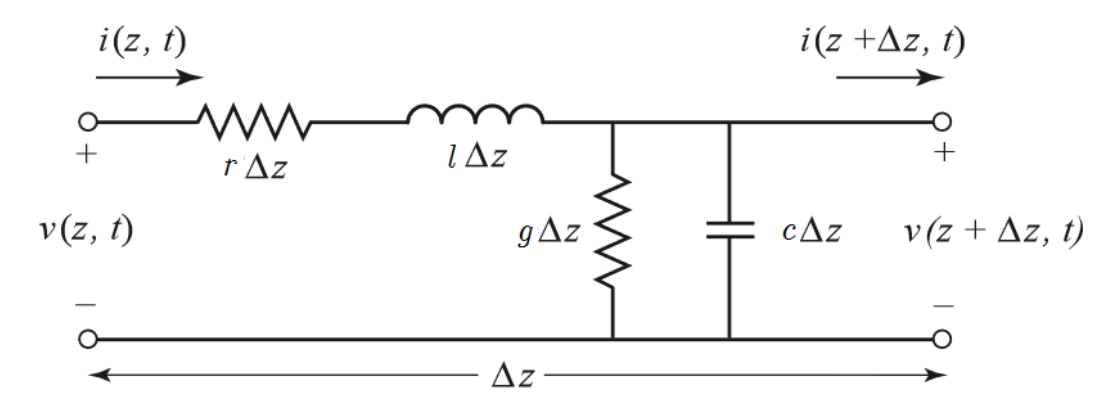
\includegraphics[width=0.4\linewidth]{chapter-theory/figs-RF/TL_lumped}
	\caption{Lumped element model of an infinitesimal short piece of a transmission line.}
	\label{fig:tllumped}
\end{figure}
We can model a transmission line, on which electromagnetic waves travel, by thinking of the EM waves as voltages and currents propagating along a distributed element circuit.
This circuit can be split into infinitesimal small elements, depicted in figure \ref{fig:tllumped}, with series resistors and inductors, and parallel conductances and capacitances.
In the following, we apply Kirchoff's laws to the circuit.
The voltage and current of this network are given by
\begin{align}
v(z,t) - r\Delta z i(z,t) - l\Delta z\frac{\partial i(z,t)}{\partial t}-v(z+\Delta z,t) &=0 \\%
i(z,t) - g\Delta z v(z+\Delta z, t) - c\Delta z\frac{\partial v(z+\Delta z,t)}{\partial t} - i(z+\Delta z,t) &=0
\end{align}
For the limit $\Delta z\rightarrow0$ these equations transform into 
\begin{align}
\frac{\partial v(z,t)}{\partial t} &= -ri(z,t)-l\frac{\partial i(z,t)}{\partial t} \\%
\frac{\partial i(z,t)}{\partial t} &= -gi(z,t)-c\frac{\partial v(z,t)}{\partial t}
\end{align}
Rewriting these equations for sinusoidal steady-state conditions and cosine-based phasors, i.e. $x(z,t) \rightarrow X(z)e^{i\omega t}$ results in the \textit{Telegrapher equations:}
\begin{align}
\frac{d^2V}{dz^2} = \gamma^2V(z) \hspace{2cm} \frac{d^2I}{dz^2} = \gamma^2I(z)
\label{eq:telegraph}
\end{align}
with the complex propagation constant
\begin{equation}
\gamma = \alpha + j\beta =\sqrt{(R+j\omega L)(G+j\omega C)}
\label{eq:gamma}
\end{equation}
where $\alpha$ is the attenuation constant and we defined $j=-i$ to avoid confusion with the current.
The solutions to these are traveling waves of the form
\begin{equation}
V(z) = V_0^+e^{-\gamma z} + V_0^-e^{\gamma z} \hspace{2cm} I(z) = I_0^+e^{-\gamma z} + I_0^-e^{\gamma z}
\label{eq:telegraph:solution}
\end{equation}
Plugging these solutions into the telegrapher equations, we get for the current on the line $I(z)=\gamma/(R+j\omega L) * V(z)$.
We can immediately see that the characteristic impedance of our transmission line is given by
\begin{align}
Z_0 \equiv \frac{V_0^+}{I_0^+}\equiv \frac{V_0^-}{I_0^-}= \frac{R+j\omega L}{\gamma} = \sqrt{\frac{R+j\omega L}{G + j\omega C}}
\end{align}
Converting this result back to the time-domain results in the following form of our voltage on the line:

\begin{align}
v(z,t) = \abs{V_0^+}\cos(\omega t-\beta z+\phi^+)e^{-\alpha z} + \abs{V_0^-}\cos(\omega t+\beta z+\phi^-)e^{\alpha z}
\end{align}

where $\phi^{\pm}$ is the phase angle of the complex voltage $V_0^{\pm}$.
Hence it is clear that the wavelength on the line is $\lambda=2\pi/\beta$, and the phase velocity $v_p=\omega/\beta=\lambda f$.
\subsection{The lossless line}
In general, the propagation constant of electromagnetic waves on a transmission line is given by the propagation constant in equation \ref{eq:gamma}.
For the lossless case $R=0$ and $G=0$ and the resulting propagation constant
\begin{align}
\gamma_\mathrm{lossless} &= j\omega\sqrt{LC} \\%
&\rightarrow \alpha=0, \; \beta=\omega\sqrt{LC}
\end{align}
For this case, we have no attenuation ($\alpha=0$) and the line impedance $Z_0=\sqrt{L/C}$ is real.
The wavelength and frequency are then simply given by
\begin{equation}
\lambda = \frac{2\pi}{\beta} = \frac{2\pi}{\sqrt{LC}} \hspace{2cm} v_p=\frac{\omega}{\beta}=\frac{1}{\sqrt{LC}}
\end{equation}

\subsection{The terminated lossless transmission line}
\begin{figure}
	\centering
	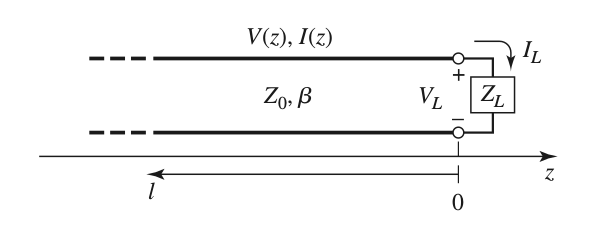
\includegraphics[width=0.4\linewidth]{chapter-theory/figs-RF/pozar_terminated_lossless}
	\caption{Sketch of a lossless transmission line terminated in a load impedance $Z_L$.}
	\label{fig:pozarterminatedlossless}
\end{figure}
Let us assume a terminated lossless line as depicted in Fig. \ref{fig:pozarterminatedlossless}.
An incident voltage wave $V_0^+ e^{-j\beta z}$ propagates from $z<0$ along the line to the right.
$V/I$ of this line is $Z_0$.
However, as the wave hits the termination, $Z_L \neq Z_0$, and a reflected wave is emitted to account for the impedance mismatch.
Using eq. \ref{eq:telegraph:solution}, the resulting impedance at $z=0$ is 
\begin{align}
Z_L=\frac{V(0)}{I(0)}=Z_0\frac{V_0^++V_0^-}{V_0^+-V_0^-} \hspace{1cm} \rightarrow V_0^-=\Gamma Z_0 \\%
\Gamma = \frac{Z_L-Z_0}{Z_L+Z_0}
\end{align} 
where we defined $\Gamma$ as the voltage reflection coefficient.

\section{Coplanar waveguides}
To confine and guide electromagnetic waves on chips, we make use of coplanar waveguides.
These consist of thin metal film of thickness $t$ on a dielectric substrate (thickness $H$).
The metal film is patterned into a center conductor of width $w$ and is separated by the ground planes by a distance $s$ (see Fig. \ref{fig:cpw-coplanar-waveguide}).
The characteristic impedance of such a CPW is given by
\begin{equation}
Z_0 = \sqrt{\frac{L'}{C'}}
\end{equation}
The electromagnetic waves in such a line are traveling with the wave velocity \begin{equation}
v=\frac{1}{\sqrt{L'C'}}=\frac{c_\mathrm{vac}}{\sqrt{\epsilon_\mathrm{eff}}}.
\end{equation}
If we assume a very thin film with large gaps, i.e. $t \ll s \ll H \rightarrow \infty$, and by defining the effective dielectric constant $\epsilon_\mathrm{eff} = \frac{1+\epsilon_r}{2}$, the transmission line parameters can all be reduced to the following expressions:
\begin{align}
C' &= 2\epsilon_0(\epsilon_r+1)\frac{K(K_0)}{K(k'_0)} \\%
L' &= \frac{\mu_0}{4}\frac{K(k'_0)}{K(k_0)} \\%
Z_0 &= \frac{c\mu_0}{\sqrt{8(\epsilon_r+1)}}\frac{K(k'_0)}{K(k_0)}\approx \frac{30\pi}{\sqrt{(\epsilon_r+1)/2}}\frac{K(k'_0)}{K(k_0)} \\%
v &= \frac{c}{\sqrt{(\epsilon_r+1)/2}}
\end{align}
\begin{figure}
	\centering
	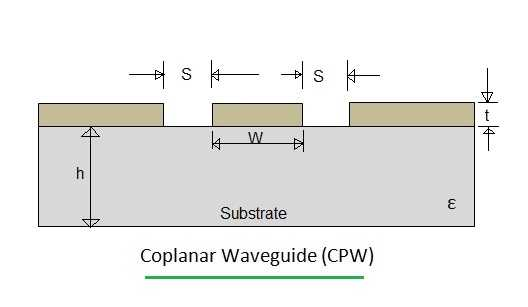
\includegraphics[width=0.3\linewidth]{chapter-theory/figs-RF/CPW-Coplanar-Waveguide.jpg}
	\caption{Cross section of a coplanar waveguide on a dielectric substrate.}
	\label{fig:cpw-coplanar-waveguide}
\end{figure}
where $K(q) = \frac{\pi}{2}\sum_{n=0}^{\infty}\left(\frac{(2n-1)!!}{(2n)!!}\right)^2 q^{2n}$ is the complete elliptic integral of the first kind, and
\begin{align}
k_0 = \frac{w}{w+2s} \hspace{2cm} k'_0 = \sqrt{1-k_0^2}.
\end{align}
Thus, it is obvious that all line parameters depend only on geometric factors, primarily on the ratio of center conductor width $w$ to gap separation $s$.


\section{Kinetic inductance}
For highly disordered superconductors, such as MoRe or NbTiN, there is an additional effect to be taken into account when analysing or designing a circuit: The so-called \textit{kinetic inductance} $L_k$. It arises naturally from the Drude model, when considering electron relaxation times comparable to the excitation frequency. This then leads to an additional inductance term from the kinetic energy of the electrons that are "lagging behind" the excitation signal. For a superconducting wire with length $l$ and crossection $A$, it is given by
\begin{eqnarray}
L_k = \frac{m}{2n_s e^2}\frac{l}{A}
\end{eqnarray}
with $n_s$ the Cooper pair density. For a CPW, $L_k$ reads
\begin{eqnarray}
L_k = g L_s = g\mu_0\lambda_m\coth\left(\frac{t}{\lambda_m}\right)
\end{eqnarray}
where $L_s$ denotes the surface inductance, $t$ the film thickness, $g=g(S,W,t)$ the geometry factor of the CPW, $\Delta_0\approx1.764\,k_BT_c$ the superconducting gap at \SI{0}{K} and $\lambda_m$ the London penetration depth at $T\rightarrow0$ as
\begin{eqnarray}
\lambda_m=\sqrt{\frac{\hbar\rho}{\pi\mu_0\Delta_0}}\approx\SI{105}{(nm)}\cdot\sqrt{\frac{\rho\si{\,(\micro\ohm\,\centi\metre)}}{T_c \si{\,(K)}}}
\end{eqnarray}
This length changes as a function of temperature according to
\begin{eqnarray}
\lambda_m(T) = \frac{\lambda_m(0)}{\sqrt{1-\left(\frac{T}{T_c}\right)^4}}
\end{eqnarray}

\subsection{Current bias cavities, or series RLC circuit capacitively coupled to one side of a transmission line}
\begin{figure}[!h]
	\centering
	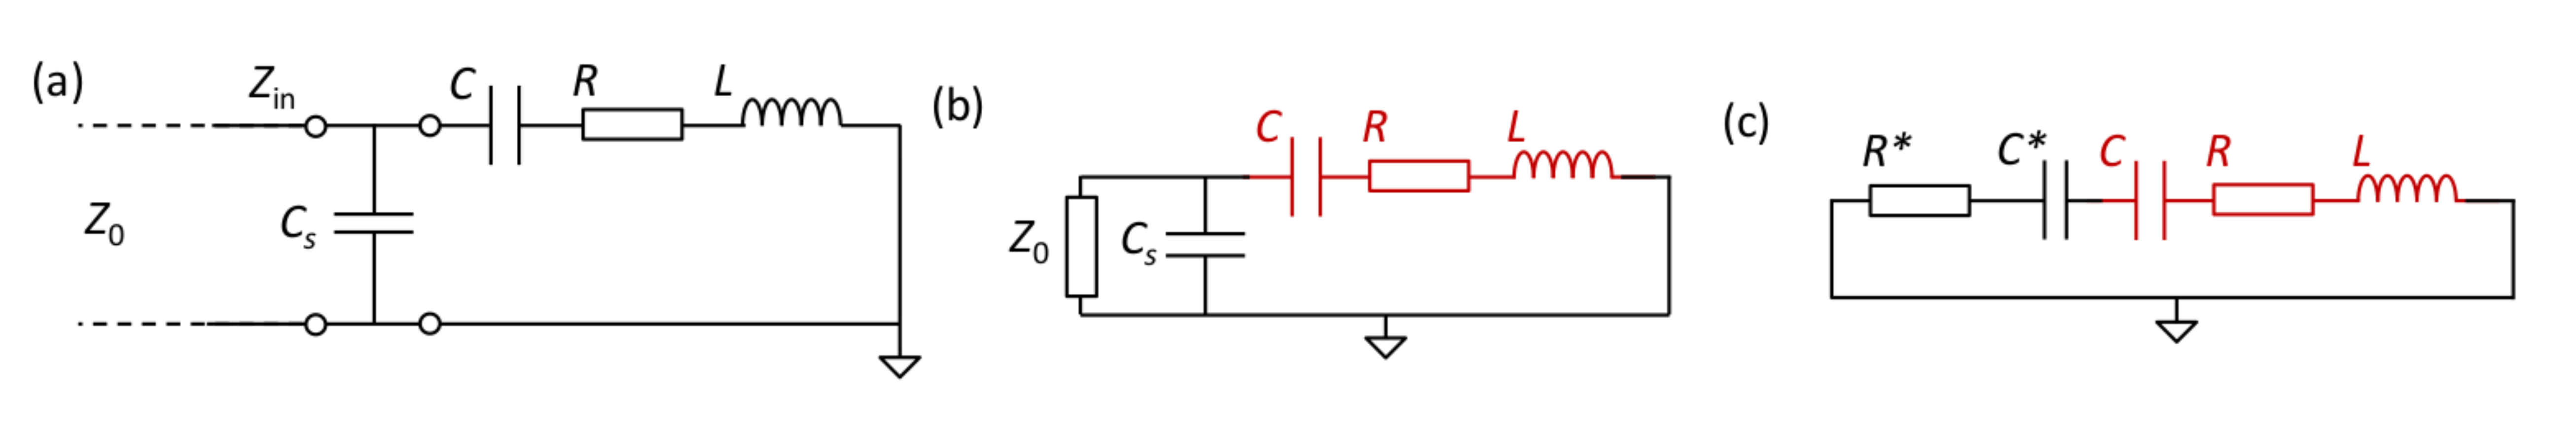
\includegraphics[width=0.7\linewidth]{chapter-theory/figs-RF/resonator_Daniel_crop}
	\caption{Lumped element model of a series RLC circuit capacitively coupled to one side of a transmission line. (a) Transmission line model. (b) Equivalent lumped element circuit. (c) Transformation to effective series circuit.}
	\label{fig:resonatordaniel}
\end{figure}

We analyze the circuit depicted in Fig. \ref{fig:resonatordaniel}. Typically we can assume $C_s\gg C$. The shunt capacitor and feedline have the total impedance
\begin{align}
Z_e = \left(\frac{1}{Z_0}+i\omega C_s\right)^{-1} = \frac{Z_0}{1+i\omega C_s} &= \frac{Z_0}{1+(\omega C_s Z_0)^2} + \frac{1}{i\omega}\frac{\omega^2 C_s Z_0^2}{1+(\omega C_s Z_0)^2} \\%
&= R^* + \frac{1}{i\omega}\frac{1}{C^*}
\end{align}
Hence we can transform the shunt capacitor and transmision line impedance into a series system together with the $RLC$-resonator. For this type of coupling, usually $\omega C_s Z_0\gg1$ aournd the resonance $\omega\approx\omega_0$. Hence, we can define these lumped elements as
\begin{align}
R^* \approx \frac{1}{\omega_0^2 C_s^2 Z_0}, \hspace{2cm}C^*\approx C_s
\end{align}
Then, for the total capacitance and resistance, we get 
\begin{align}
R_\mathrm{tot} = R+R^*, \hspace{2cm} C_\mathrm{tot}=\frac{C C_s}{C + C_s}
\end{align}

This lumped element circuit has the resonance frequency
\begin{align}
\omega_0 = \frac{1}{\sqrt{LC_\mathrm{tot}}} = \sqrt{\frac{C+C_s}{L C C_s}}
\end{align}
We can see that the coupling capacitor $C_s$ shifts the resonance frequency upwards, compared to the bare resonance frequency.
The total quality factor,
\begin{equation}
Q_L = \frac{1}{\omega_0 R_\mathrm{tot}C_\mathrm{tot}} = \left(\frac{1}{Q_\mathrm{int}} + \frac{1}{Q_\mathrm{ext}}\right)^{-1}
\end{equation}
can be separated into its internal and external components
\begin{align}
Q_\mathrm{int} &= \frac{C+C_s}{\omega_0 R C C_s}, \hspace{2cm} Q_\mathrm{ext} = \frac{C+C_s}{\omega_0 R^* C C_s} = \frac{\omega_0 Z_0 C_S (C+C_s)}{C} \\%
\kappa_\mathrm{ext} &= \frac{\omega_0}{Q_\mathrm{ext}} = \frac{\omega_0 R C C_s}{C+C_s}, \hspace{2cm} \kappa_\mathrm{ext} = \frac{\omega_0}{Q_\mathrm{ext}} = \frac{C}{Z_0 C_s (C+C_s)}
\end{align}
We can now calculate the complete input impedance of this circuit for the lossless case, i.e. $R=0$:
\begin{align}
\frac{1}{Z_\mathrm{in}}&=\left(i\omega L + \frac{1}{i\omega C}\right)^{-1} + i\omega C_s = i\frac{\omega(C+C_s)-\omega^3LCC_s}{1-\omega^2LC} \\%
&=i\omega\frac{C+C_s}{1-\omega^2LC}\left(1-\frac{\omega^2}{\omega_0^2}\right), \hspace{2cm} \omega_0=\frac{C+C_s}{LCC_s} \\%
&\approx2i\frac{C_s(C+C_s)}{C}\Delta\omega \\%
&\longrightarrow Z_\mathrm{in} \approx \frac{C}{C_s (C+C_s)}\frac{1}{\kappa_\mathrm{int}+2i\Delta\omega}.
\end{align}

With this, we get for the reflection parameter
\begin{equation}
\Gamma = \frac{Z_\mathrm{in}-Z_0}{Z_\mathrm{in}+Z_0}\approx\frac{\kappa_\mathrm{ext}-\kappa_\mathrm{int}-2i\Delta\omega}{\kappa_\mathrm{ext}+\kappa_\mathrm{int}+2i\Delta\omega}.
\end{equation}

\section{The Duffing oscillator}

\subsection{Analytical Ansatz}
As we have seen, Josephson junctions act as nonlinear inductors, hence adding nonlinearity, or anharmonicity, to an electrical circuit.
When the circuit is driven with low enough input power, the nonlinearity can be neglected.
In this case, the circuit can be described well by a driven harmonic oscillator,
\begin{align}
\ddot{x} + \delta \dot{x} + \alpha x = \gamma \cos(\omega t),
\end{align}
with the time-dependent displacement  $x=x(t)$, stiffness $\alpha$, damping $\delta$, drive amplitude $\gamma$ and drive frequency $\omega$.
All variables are assumed to be positive and real.
However, for most cases it is important to account for the anharmonicity.
The generalized mathematical model which describes such a circuit is the Duffing equation with the following equation of motion (EOM)\cite{hamelGeorgDuffingIngenieur1921}:
\begin{align}
\ddot{x} + \delta \dot{x} + \alpha x + \beta x^3 = \gamma \cos(\omega t),
\end{align}
with the anharmonicity $\beta$.

In fact, there exists an algebraic equation describing the amplitude response\cite{jordanNonlinearOrdinaryDifferential2007}:
\begin{align}
\left[ \left( \omega^2-\alpha-\frac{3}{4}\beta x^2 \right)^2 + \left( \delta\omega \right)^2 \right] x^2 = \gamma^2
\label{eq:Duffing-analytical}
\end{align}
We plot the solutions to a set of parameters ($\alpha=\gamma=1,\delta=0.1$) in Fig.\ref{fig:duffing}.

\begin{figure}
	\centering
	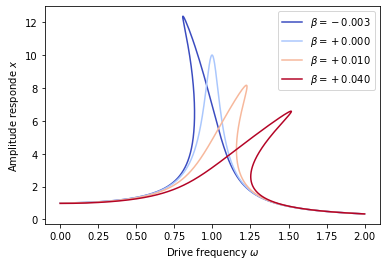
\includegraphics[width=0.7\linewidth]{chapter-theory/figs-general/duffing}
	\caption{Frequency response of Duffing oscillators for various nonlinearities and $\alpha=\gamma=1,\delta=0.1$, calculated from Eq.\ref{eq:Duffing-analytical}}
	\label{fig:duffing}
\end{figure}

\subsection{Intuitive Ansatz}
We can also take a more intuitive Ansatz to the above problem from which we can already gain qualitative information.
Let us assume the Duffing equation describes a mass on a (nonlinear) spring driven by a periodic external force.
Compared to the linear case with $F_r=kx$, the new restoring force is now given by 
\begin{align}
F_r = k^\prime x = (\alpha +\beta x^2)x.
\end{align}
For $\beta>0$, the spring is stiffened, for $\beta<0$ the spring is softened.
Quantitatively, the sign of $\beta$ does not have any effect on the behaviour of the circuit for frequency shifts small compared to the resonance frequency of the circuit.
Following first order perturbation theory, let us assume 
\begin{align}
x=x_0 \cos(\omega t)% + x_1\cos(3\omega t) + \dots
\end{align}
to be the solution of the unperturbed EOM.
If we insert this into the equation for the restoring force, we need to first calculate
\begin{align}
x^2(t) = x_0^2\cos^2(\omega t) = x_0^2\frac{1}{2}(1+2\cos(2\omega t))
\end{align}
Compared to $\cos(\omega t)$, the time average of $\cos(2\omega t)$ is zero.
Thus, the restoring force is given by
\begin{align}
F_r=k^\prime x \approx \left(k+\frac{\beta x_0^2}{2}\right)x
\end{align}
and the corresponding resonance frequency
\begin{align}
\omega \approx \omega_0 + \diff{\omega}{k}\Delta k \approx \omega_0 + \frac{\omega_0}{2}\frac{\Delta k}{k} = \omega_0 \left(1+\frac{\beta x_0^2}{4k}\right).
\end{align}
We see that the resonance frequency of the unperturbed system experiences a shift proportional to $\beta$ and the square of the position, $x_0^2$.

%\bibliography{dissertation}

\references{dissertation}

